\chapter{Background Information and Literature Review}
\label{cha:2}

\section{Media Bias}

Allsides \cite{allsides-2022-bias-definition} defines media bias as "The tendency of news media to report in a way that reinforces a viewpoint, world-view, preference, political ideology, corporate or financial interests, moral framework, or policy inclination, instead of reporting in an objective way (simply describing the facts)". Media bias has existed and been researched since the 1950s \cite{white-1950-case-study-selection-news}.

\begin{figure}[htbp]
    \centering
    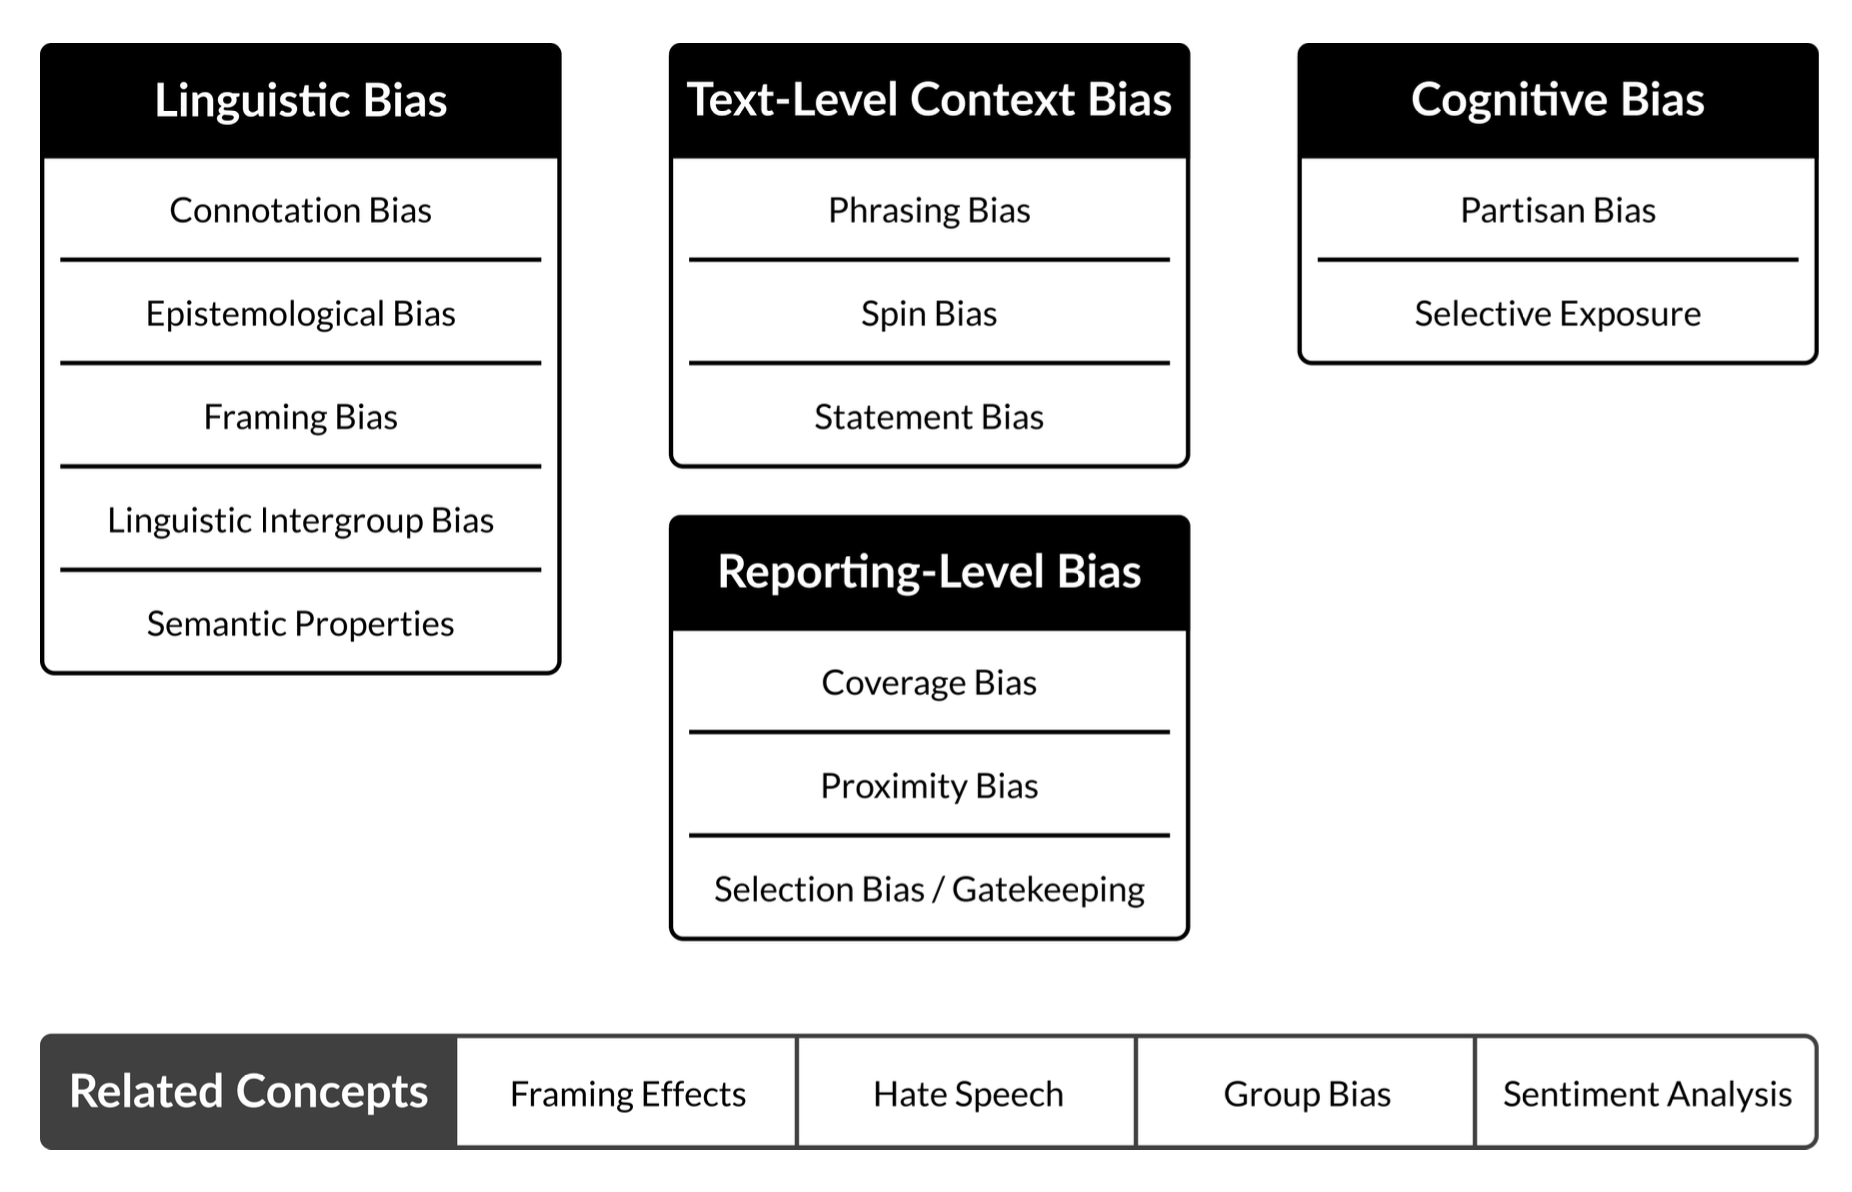
\includegraphics[width=0.9\linewidth]{images/bias-types-taxonomy.png}
    \caption{Media bias types as defined in The Media Bias Taxonomy \cite{spinde-2024-taxonomy}}
    \label{fig:media-bias-taxonomy}
\end{figure}

Many works and authors have tried to categorise media bias based on its types and characteristics \cite{rodrigo-2024-systematic-review-media-bias,eberl-2017-bias-political,spinde-2024-taxonomy,allsides-media-bias-types}. This project will follow The Media Bias Taxonomy by Spinde et al. (Figure \ref{fig:media-bias-taxonomy}), focusing on \textbf{Text-level Context Bias}, which pertains to the context of a text and the manner in which it is conveyed \cite{spinde-2024-taxonomy}.

\begin{figure}[htbp]
    \centering
    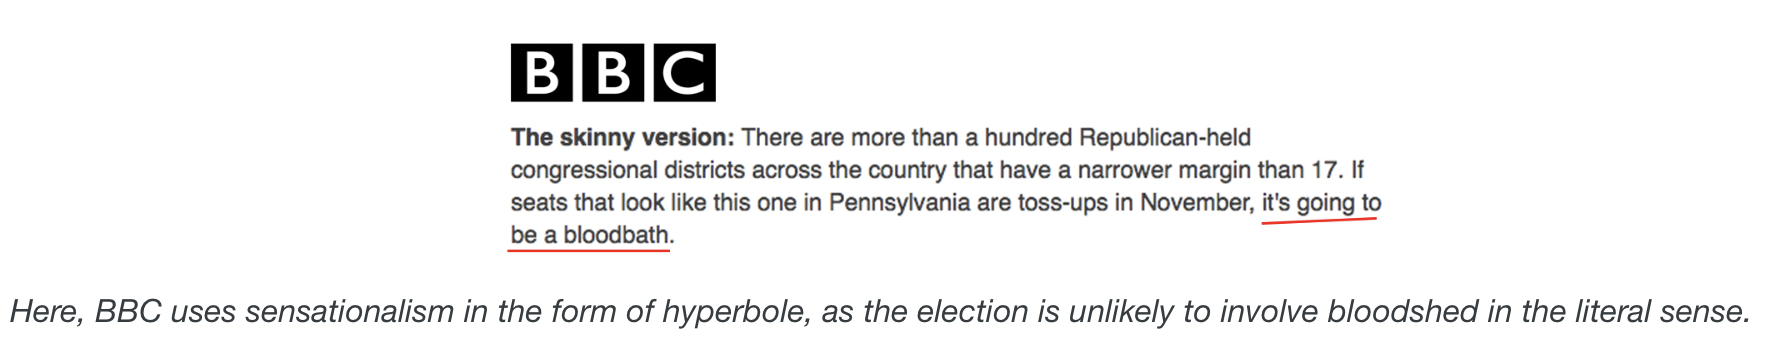
\includegraphics[width=0.95\linewidth]{images/phrasing_bias_example.png}
    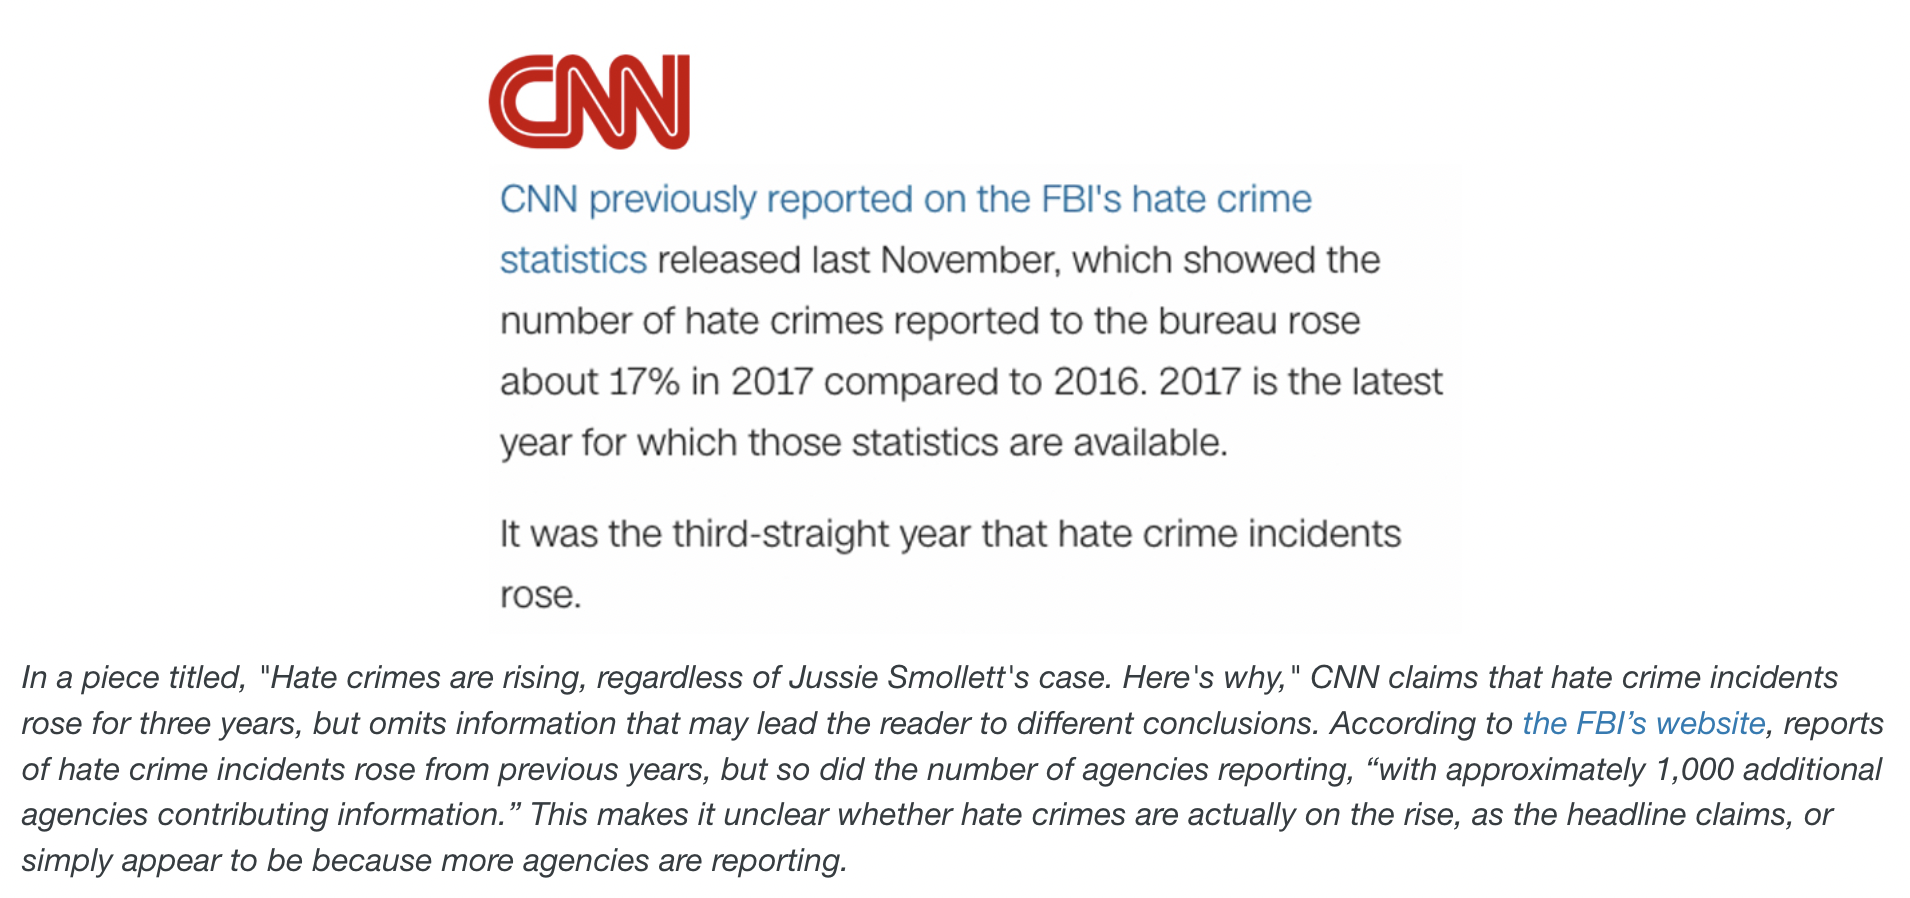
\includegraphics[width=0.95\linewidth]{images/spin_bias_example.png}
    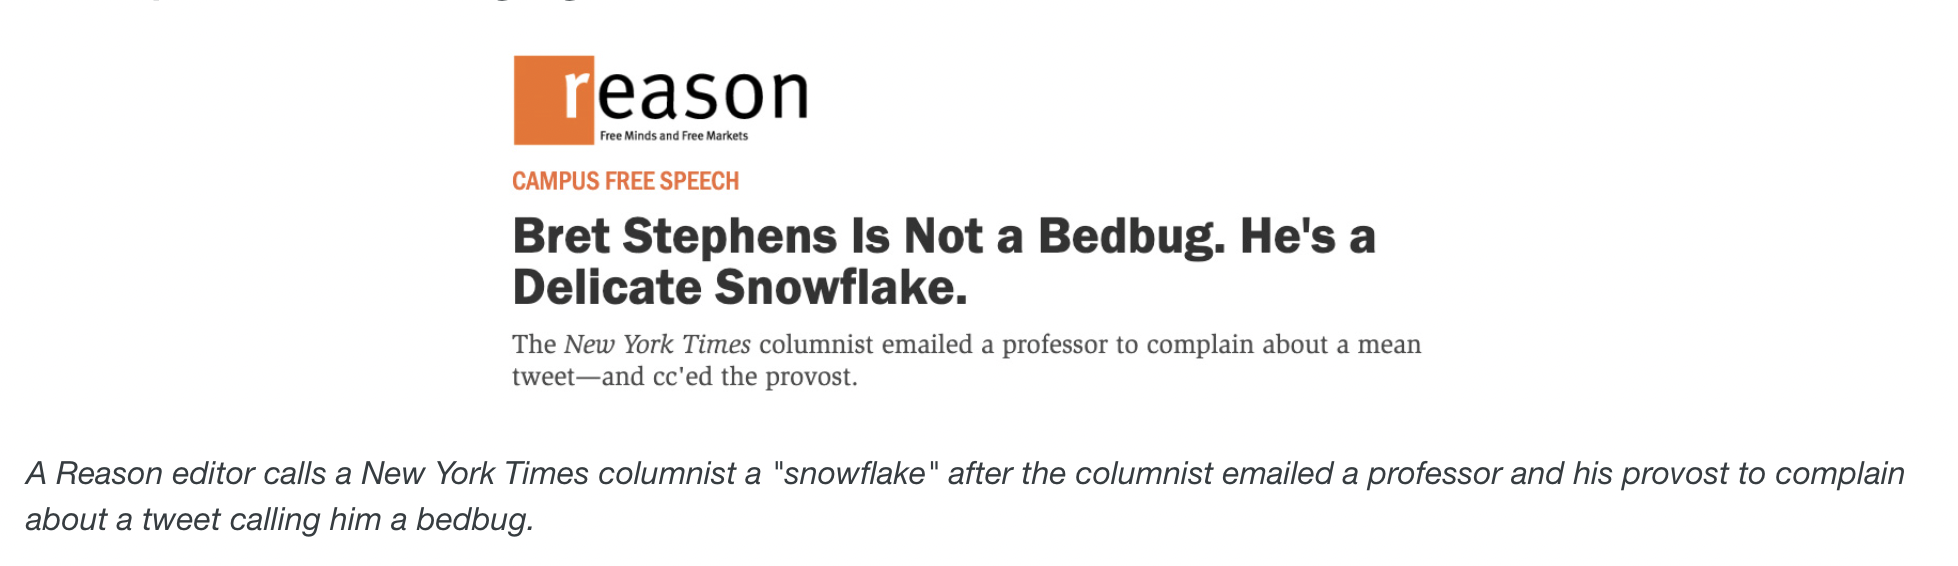
\includegraphics[width=0.95\linewidth]{images/statement_bias_example.png}
    \caption{Example of phrasing bias (top), spin bias (middle), and statement bias (bottom) \cite{allsides-media-bias-types}}
    \label{fig:bias-examples}
\end{figure}

Figure \ref{fig:bias-examples} shows examples taken from the Allsides website \cite{allsides-media-bias-types} referring to the three types of text-level context bias: phrasing bias, spin bias, and statement bias. Phrasing bias is characterised by the use of provocative, inflammatory, or non-neutral language, using words that may evoke specific feelings or emotions in the reader \cite{spinde-2024-taxonomy,hube-2019-neural-biased-language}. The top article snippet in Figure \ref{fig:bias-examples} shows the phrase "it's going to be a bloodbath". The phrase can be considered phrasing bias as it evokes a violent image and may lead readers to perceive the election as extremely chaotic or violent, even though it is not literal. Spin bias is introduced when essential information is omitted from the narrative, or when irrelevant information is added instead \cite{spinde-2024-taxonomy}, often as an effort to craft a memorable story \cite{mullainathan-2002-media-bias}. The middle article in Figure \ref{fig:bias-examples} purposefully omitted the crucial information that the number of agencies reporting hate crime incidents has also increased. This creates a false narrative that hate crimes are on the rise, despite the possibility that the increase in reported incidents might be attributed due to higher number of reporting agencies. Statement bias occurs when media personnel insert their personal views into the content, resulting in certain news being presented in a manner that is more or less favourable towards a particular view or position \cite{spinde-2024-taxonomy,d-alessio-2000-meta-analysis}. The sentence "He's a delicate snowflake" shown in the example (Figure \ref{fig:bias-examples} bottom article) is clearly a personal opinion of the author of the post.

\begin{figure}[htbp]
    \centering
    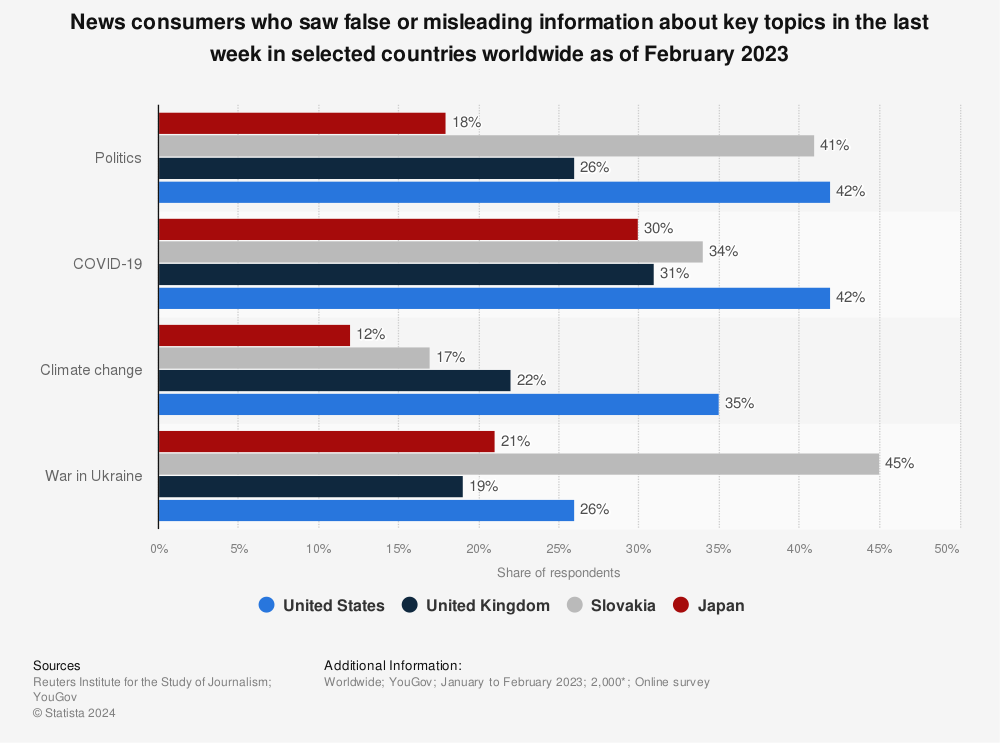
\includegraphics[width=0.9\linewidth]{images/statistic_id1317019_consumers-witnessing-false-information-on-certain-topics-worldwide-2023.png}
    \caption{The rate of news consumers witnessing false or misleading information on several recent key topics in February 2023 \cite{reuters-2023-false-info}}
    \label{fig:consumers-witnessing-false-information-on-certain-topics-worldwide-2023}
\end{figure}


\begin{figure}[htbp]
    \centering
    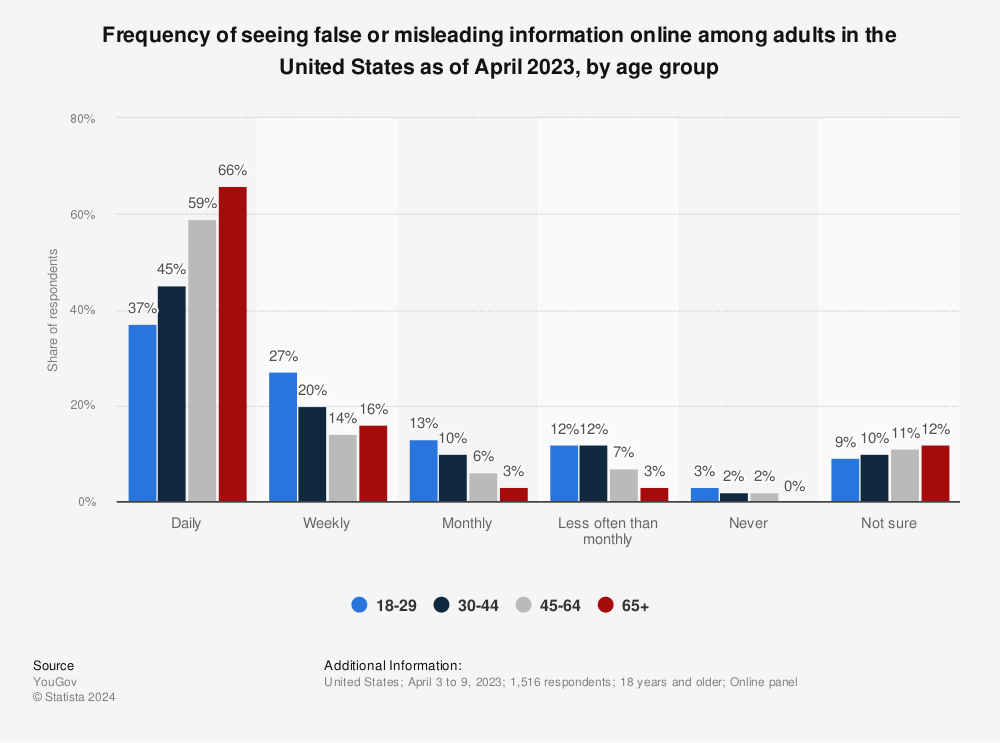
\includegraphics[width=0.9\linewidth]{images/statistic_id1462057_frequency-of-seeing-false-information-online-in-the-us-2023-by-age-group.png}
    \caption{Frequency of seeing false or misleading information online in the United States as of April 2023, by age group \cite{yougov-2023-frequency}}
    \label{fig:frequency-of-seeing-false-information-online-in-the-us-2023-by-age-group}
\end{figure}


Media bias and misinformation are particularly prominent and visible within the United States, compared to other countries. Based on surveys from Reuters \cite{reuters-2023-false-info} and YouGov \cite{yougov-2023-frequency} (Figure \ref{fig:consumers-witnessing-false-information-on-certain-topics-worldwide-2023} and Figure \ref{fig:frequency-of-seeing-false-information-online-in-the-us-2023-by-age-group}), the United States is shown to have the highest rate of encountering false or misleading information related to politics, COVID-19, and climate change. Nearly half of the respondents reported seeing such information in the week prior to the survey. Additionally, most adults across all age groups reported seeing false or misleading information on a \textbf{daily} basis.

Furthermore, Trust in news media in the US is at an all-time low, declining consistently and significantly over the past 20 years \cite{pew-2021-partisan-divides, gallup-knight-2020-american-views, reuters-2023-digital-news-report}. Approximately half of Americans believe that the media is significantly responsible for the political divisions within the United States, with a growing number of Americans losing faith in the media's objectivity and perceiving it as actively engaging in ideological wars \cite{gallup-knight-2020-american-views}. Reuters Institute also reported less than half of their respondents (40\%) generally trust the majority of news sources, with the US ranked on 29\textsuperscript{th} out of 40 countries (32\%) in terms of trust \cite{reuters-2023-digital-news-report,reuters-2023-trust} (full figure shown in Figure \ref{fig:trustworthiness-of-news-media-worldwide-2023}).

\begin{figure}[htbp]
    \centering
    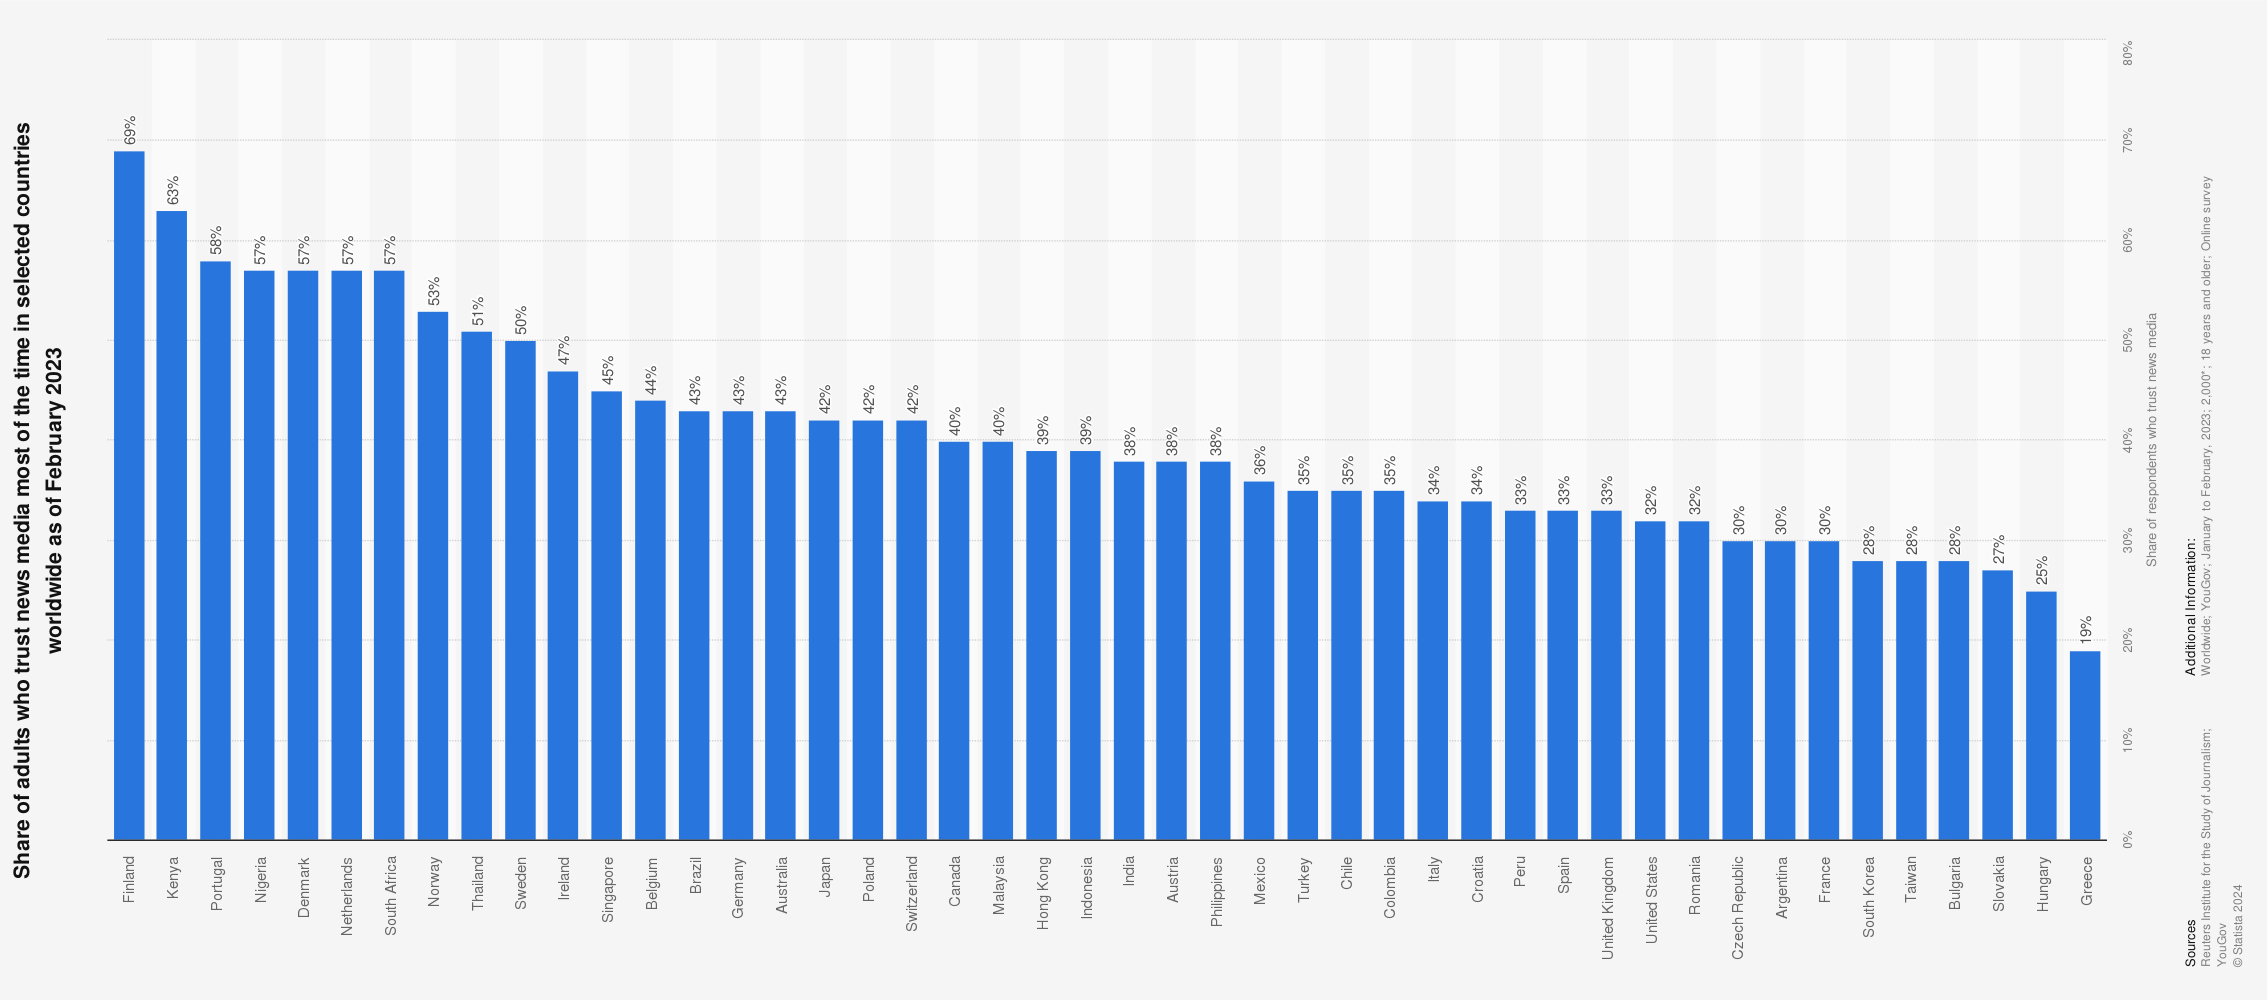
\includegraphics[width=0.6\linewidth]{images/statistic_id308468_trustworthiness-of-news-media-worldwide-2023.png}
    \caption{Trustworthiness of news media worldwide, as of February 2023 \cite{reuters-2023-trust}}
    \label{fig:trustworthiness-of-news-media-worldwide-2023}
\end{figure}

These findings highlight the severity of media bias in the United States. Given that the majority of resources on media bias are generally US-centric \cite{allsides,adfontes}, it is practically efficient to focus this project on US-based articles and domains. Given that the majority of research and resources on media bias are typically focused on the US \cite{allsides, adfontes,rodrigo-2024-systematic-review-media-bias}, it is both practical and reasonable for this project to concentrate on US-based articles and domains.

\begin{comment}
Objectivity itself is defined by Cambridge Dictionary as "the fact of being based on facts and not influenced by personal beliefs or feelings" \cite{cambridge-dictionary-objectivity}.

(Journalism has abandoned the idea of seeking neutrality and objectivity, aiming instead to adopt a more engaged and committed approach) Objectivity in the media has been rejected both as an impossible standard and as an undesirable norm. \cite{boudana-2011-journalistic-objectivity}.

A survey of journalists from the United States, Great Britain, Germany, Italy, and Sweden found evidence that journalists' personal beliefs substantially influence their news decisions, expressed within the stories they choose and the statements they write \cite{patterson-donsbach-1996-news-decisions}.

Panagopoulos' study \cite{panagopoulos-2020} revealed systemic biases leaning towards Democratic candidates during national and state levels pre-election polls conducted during the 2020 U.S. general election cycle. Rafail et al. \cite{rafail-2018-tea-party} examined 201,678 media documents from Tea Party organizations, Fox News, MSNBC, and 785 newspapers, revealing significant differences in how the Tea Party frames itself compared to how other media sources frame the movement, MSNBC portrays it as the worst aspect of the Republican Party, while Fox News sees it as the best, sharply in contrasts with how activists frame the movement as conservative but not strictly Republican, often clashing with Republican Party goals.

An analysis by Pew Research Center \cite{pew-2021-election2020} found that miscalculations observed in the 2020 U.S. election polls would adjust public opinion on issues by an average of just under 1 percentage point. Although errors of such scale would not have produced substantial differences on the American public opinions, this shows the underlying bias within polls specifically and the failure of accurately representing surveys.

Readers themselves are not exempt from bias, as they are known to prefer to pick, follow, and consume articles that align with their own beliefs and ideology, an issue known as filter bubble \cite{lim-2018-understanding} or selective exposure \cite{spinde-2024-taxonomy}. This incident reinforces existing biases and limits exposure to diverse perspectives, creating echo chambers that hinder critical thinking and informed decision-making. The combination of media bias and filter bubbles can distort reality, perpetuate misinformation, and deepen societal divisions.
\end{comment}

\section{Word Embeddings}

\begin{figure}[htbp]
    \centering
    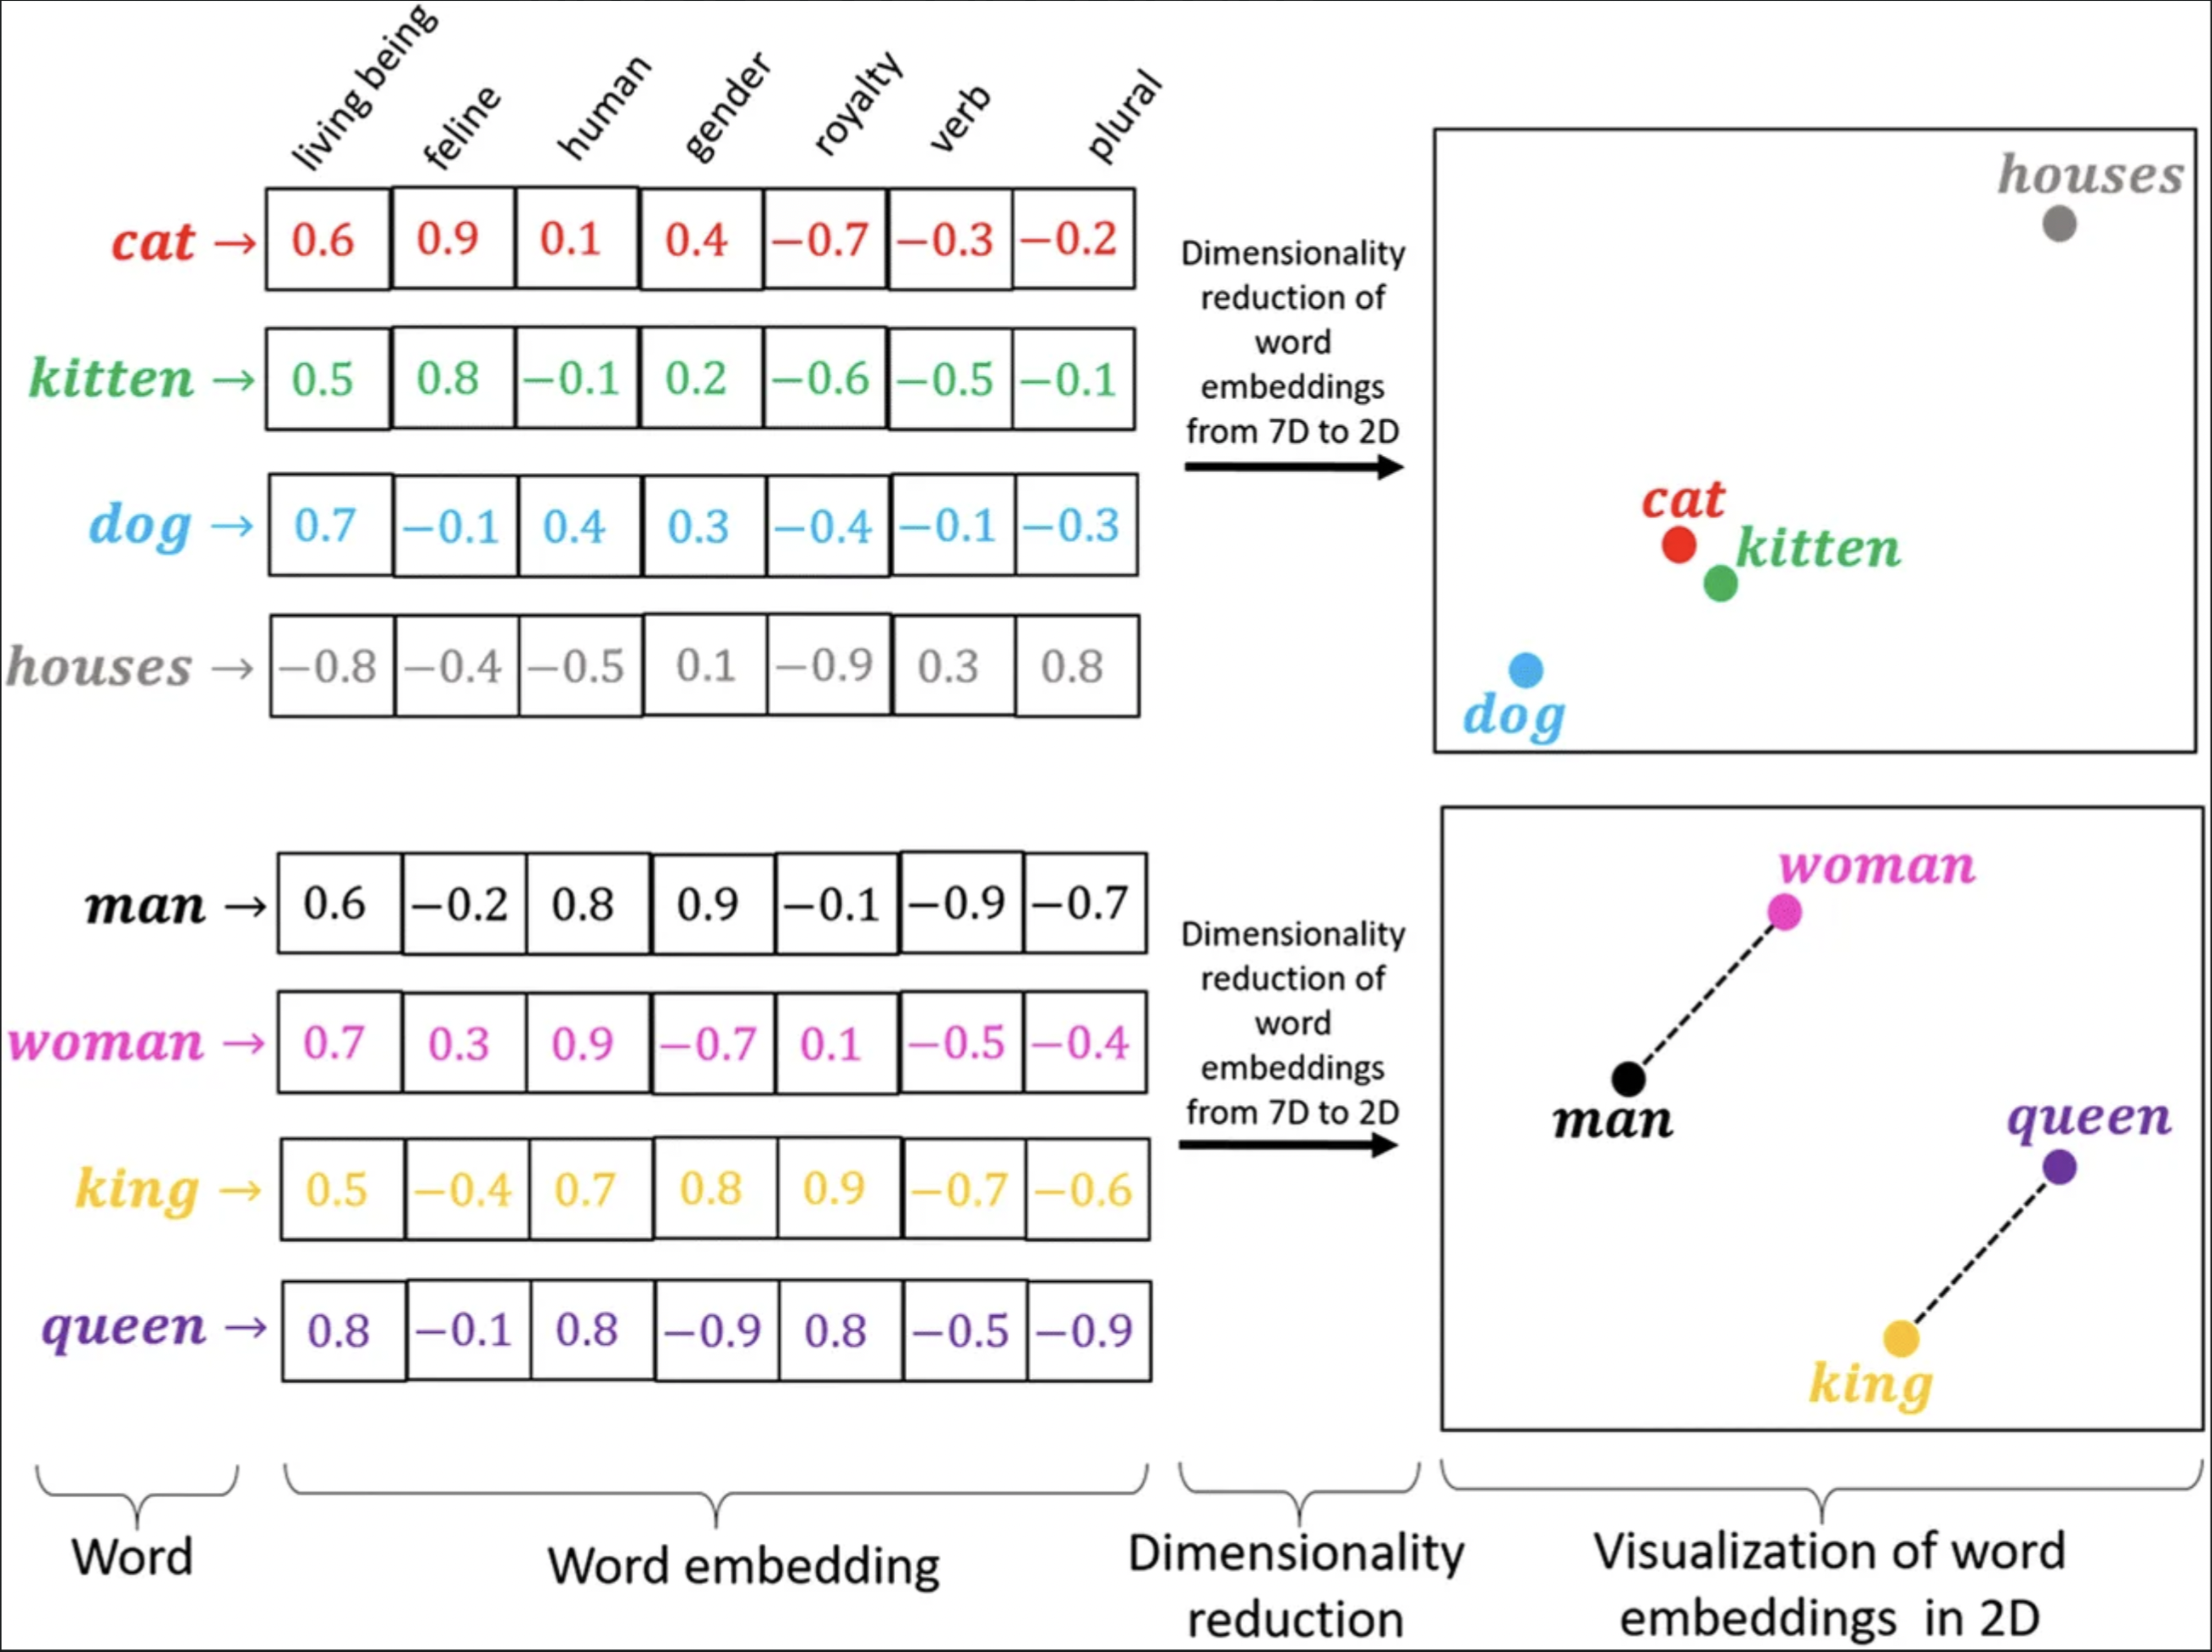
\includegraphics[width=0.9\linewidth]{images/word_embeddings.png}
    \caption{Word embeddings visualisation \cite{narayanan-2019-word-embeddings}}
    \label{fig:word-embeddings}
\end{figure}

Word embeddings are a way to represent words in a continuous vector space where words with similar meanings are placed close to each other, thereby capturing semantic relationships between words. This approach gained significant popularity with the introduction of \textit{word2vec} as a method to generate word embeddings \cite{mikolov-2013-embeddings}. Most Natural Language Processing (NLP) tasks approaches still inherently rely on word embeddings to represent textual data, often serving as the initial input to models. An example of word embeddings is visualised in Figure \ref{fig:word-embeddings}.


\section{MultiLayer Perceptron (MLP)}

\begin{figure}[htbp]
    \centering
    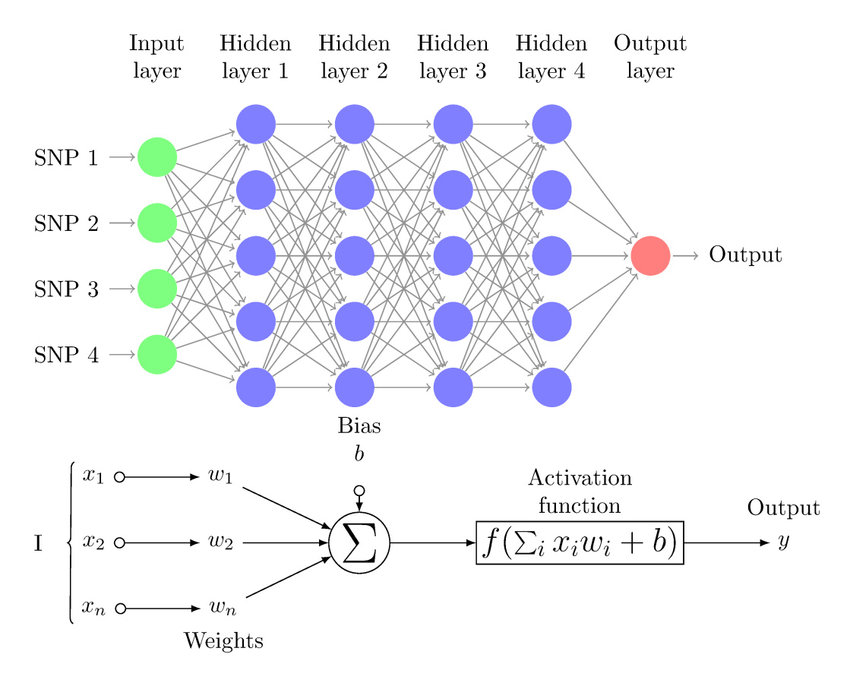
\includegraphics[width=0.9\linewidth]{images/mlp.png}
    \caption{MultiLayer Perceptron visualisation \cite{perez-enciso-2019-guide}}
    \label{fig:mlp}
\end{figure}

A MultiLayer Perceptron (MLP) is a fully connected Artificial Neural Network (ANN) that consists of single or multiple hidden layers, illustrated in Figure \ref{fig:mlp}. Hidden layers refer to the collection of neurons that are between the input and output layers, transforming data from layer to layer \cite{uzair-2020-hidden-layers}. The weighted sum (\( \mathbf{z} \)) in a hidden layer of a neural network is computed as follows (Equation \eqref{eq:z}):

\begin{equation}
    \label{eq:z}
    \mathbf{z} = \mathbf{W}\mathbf{x} + \mathbf{b}
\end{equation} where \( \mathbf{x} \) is the input vector, \( \mathbf{W} \) is the weight matrix, \( \mathbf{b} \) is the bias vector. After computing \( \mathbf{z} \), an activation function \( f \) is applied element-wise to produce the output \( \mathbf{h} \) (Equation \eqref{eq:h}):

\begin{equation}
    \label{eq:h}
    \mathbf{h} = f(\mathbf{z})
\end{equation}

MLP is widely used due to its ability to introduce non-linearity into the model, allowing the network to approximate complex functions that are beyond the capability of simple linear models. By integrating multiple hidden layers with non-linear activation functions, MLP can learn intricate patterns and relationships within data, making them suitable for a wide range of machine learning tasks. This flexibility is pivotal in capturing the nuanced and intricate structures inherent in real-world datasets, thereby enhancing the model's predictive accuracy and generalisation capabilities.


\section{Long Short-Term Memory (LSTM)}

\begin{figure}[htbp]
    \centering
    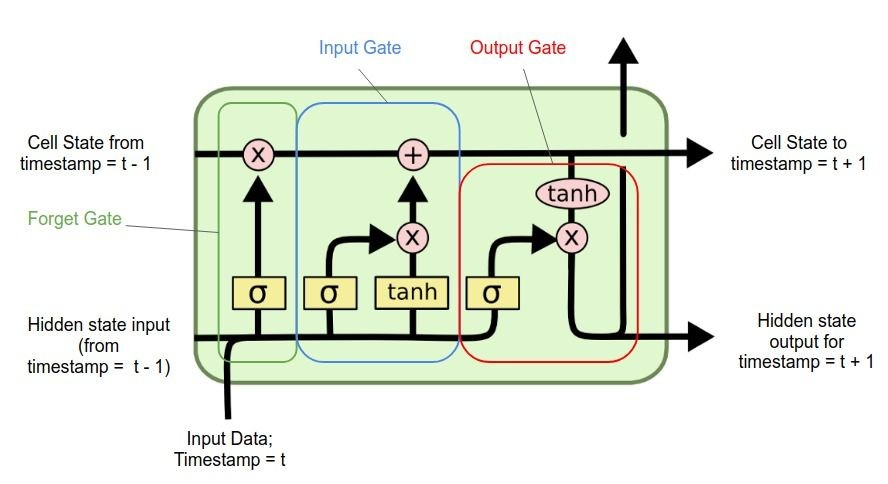
\includegraphics[width=0.9\linewidth]{images/lstm.jpeg}
    \caption{LSTM architecture \cite{rahman-2023-lstm-networks}}
    \label{fig:lstm}
\end{figure}

LSTM \cite{hochreiter-1997-lstm} is a type of Recurrent Neural Network (RNN) architecture designed to address the vanishing gradient problem and capture long-term dependencies in sequential data. It incorporates two fundamental components: memory cells and gates. Memory cells maintain a cell state, which can store information over long sequences and allows the model to retain information for longer durations compared to traditional RNNs. Gates control the flow of information into and out of the memory cell, controlled by sigmoid and tanh activation functions, which regulate the information flow based on the input data and the current state. Figure \ref{fig:lstm} shows the full architecture of a LSTM block.


\section{Transformer and Large Language Model (LLM)}

\begin{figure}[htbp]
    \centering
    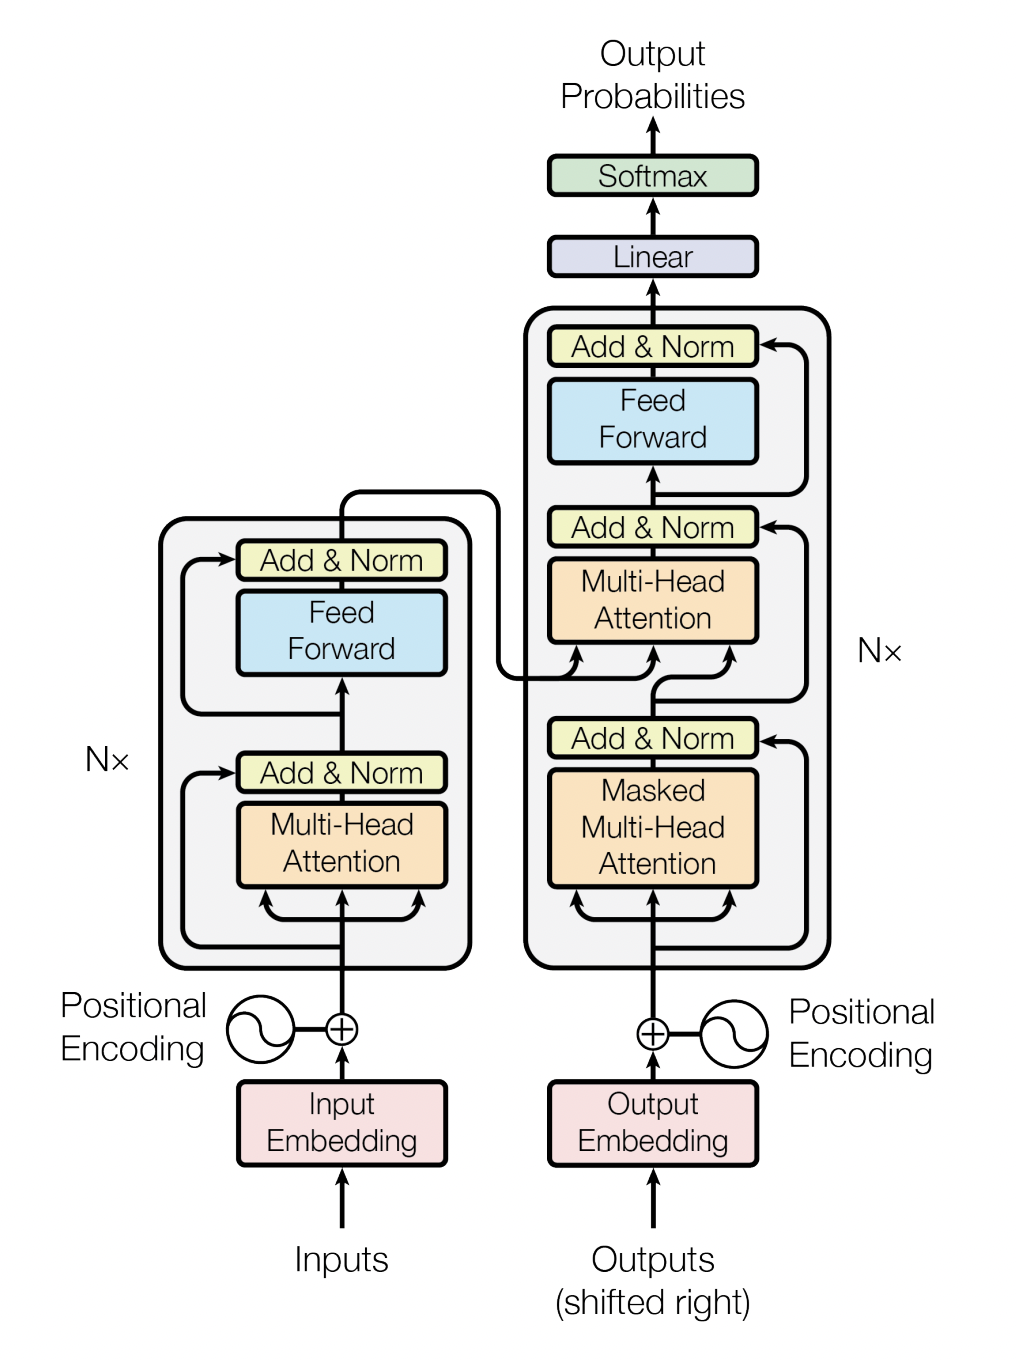
\includegraphics[width=0.7\linewidth]{images/transformer.png}
    \caption{Transformer visualisation \cite{vaswani-2023-attention}}
    \label{fig:transformer}
\end{figure}

The Transformer architecture relies entirely on attention mechanism to capture global dependencies across input and output sequences, allowing for unprecedented levels of parallelisation instead of sequential processing \cite{vaswani-2023-attention}. Their introduction marks a fundamental shift away from traditional sequence-based models like recurrent neural networks (RNNs) and convolutional neural networks (CNNs), offering unparalleled advancements in handling long-range dependencies and contextual information. Their effectiveness stems from the attention mechanism, specifically through self-attention and multi-head attention mechanisms, defined in Equation \eqref{eq:attention} and \eqref{eq:multihead} \cite{vaswani-2023-attention}. These mechanisms allow the network to weigh and prioritise relevant information across sequences, capturing intricate relationships and semantic nuances.

LLMs are artificial neural networks that utilise the transformer architecture, designed to understand and generate human language. They are trained on vast amounts of diverse text data using unsupervised learning techniques, often containing millions or even billions of parameters. Two of the most popular and widely used LLMs are \textbf{Bidirectional Encoder Representations from Transformers (BERT)} \cite{devlin-2019-bert}, comprised of 110 million parameters, and GPT, particularly GPT-4 \cite{openai-2024-gpt4}, which is reported to have an astonishing 1.76 trillion parameters, based on a report by SemiAnalysis in 2023 \cite{semianalysis-gpt4}.

\textbf{Fine-tuning} is a way to optimise pre-trained LLMs to for specific tasks or domains, aiming to achieve improved inference quality with limited resources. \cite{oracle-finetuning-blog}. During this process, the model weights are adjusted based on the training data for the downstream task, allowing the model to adapt its pre-trained representations to the specific requirements of the task. This approach leverages the powerful pre-trained representations from LLMs and adapts them with relatively small amounts of task-specific training data. It has become a widely common and popular technique for performing various NLP tasks due to its effectiveness in improving performance over traditional models.

\begin{figure}[htbp]
    \centering
    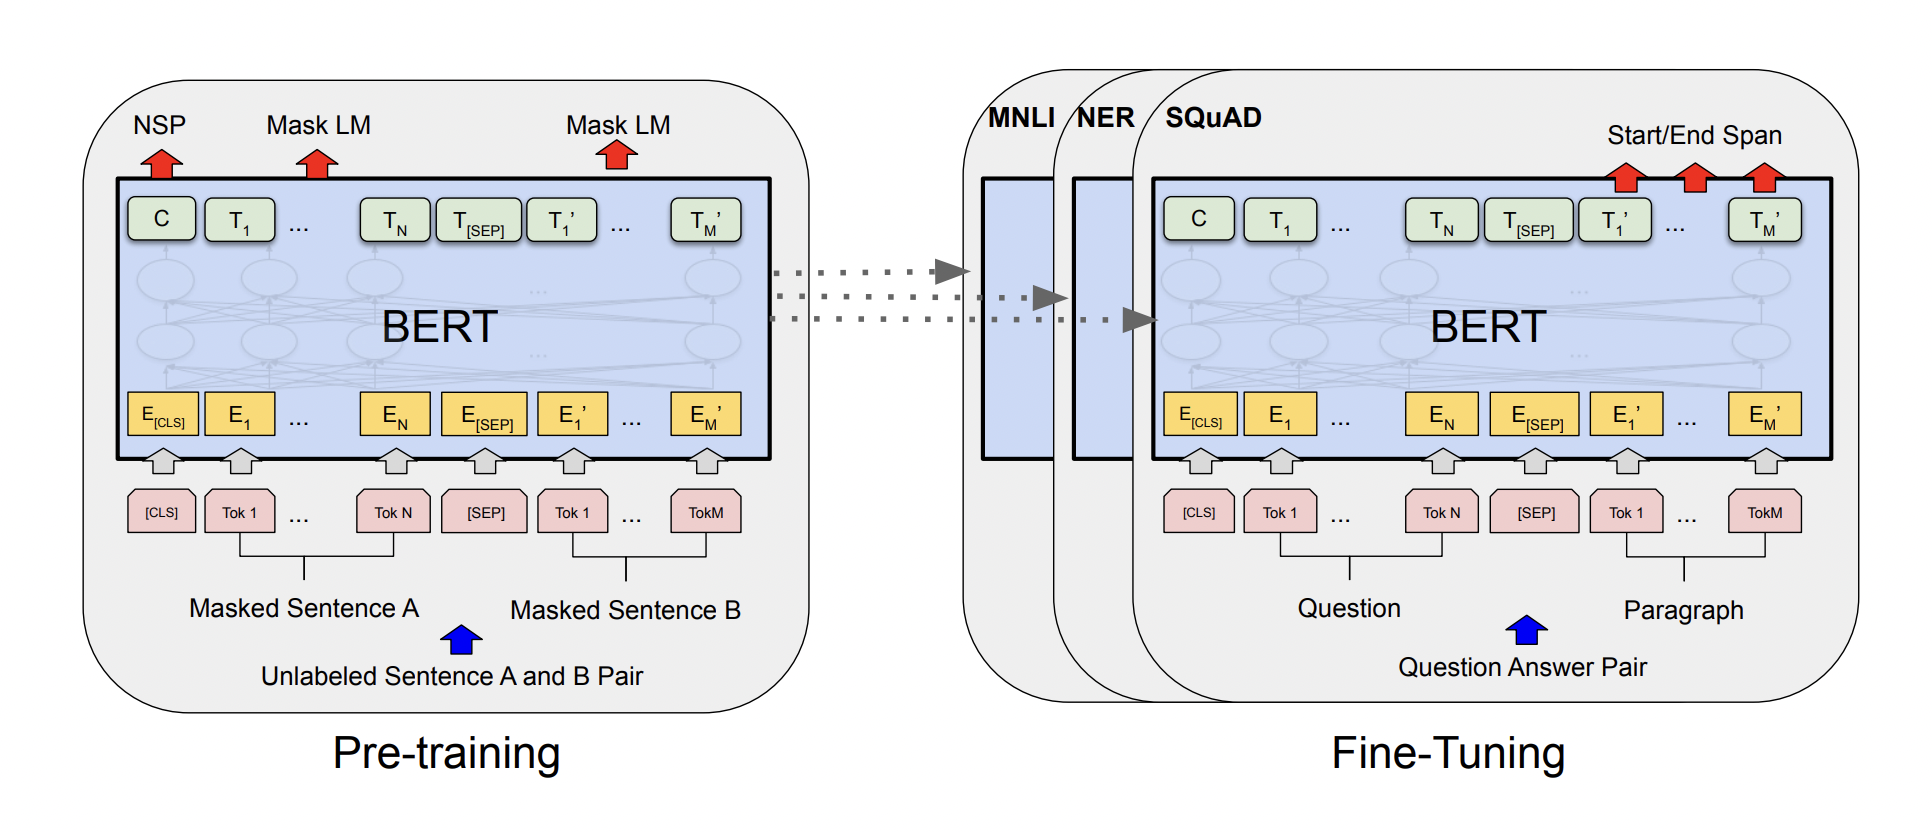
\includegraphics[width=0.9\linewidth]{images/bert_finetuning.png}
    \caption{BERT pre-training and fine-tuning procedures \cite{devlin-2019-bert}}
    \label{fig:bert_finetuning}
\end{figure}

\begin{equation}
    \label{eq:attention}
    \text{Attention}(\mathbf{Q}, \mathbf{K}, \mathbf{V}) = \text{softmax}\left( \frac{\mathbf{Q}\mathbf{K}^\top}{\sqrt{d_k}} \right) \mathbf{V}
\end{equation}

\begin{equation}
    \label{eq:multihead}
    \text{MultiHead}(\mathbf{Q}, \mathbf{K}, \mathbf{V}) = \text{Concat}(\text{head}_1, \ldots, \text{head}_h) \mathbf{W}^O
\end{equation}
where
\[
    \text{head}_i = \text{Attention}(\mathbf{Q} \mathbf{W}^Q_i, \mathbf{K} \mathbf{W}^K_i, \mathbf{V} \mathbf{W}^V_i)
\]

Transformers and LLMs have sparked a revolution in the domain of Artificial Intelligence (AI), having achieved remarkable successes across diverse fields such as natural language processing, computer vision, and audio processing \cite{lin-2022-survey-transformers}. They have single-handedly catalysed the emergence of a new era in AI capabilities observed today, predicted to have an even greater influence than the Industrial and digital revolutions combined \cite{makridakis-2017-ai-revolution}.

\section{MAGPIE}

\begin{figure}[htbp]
    \centering
    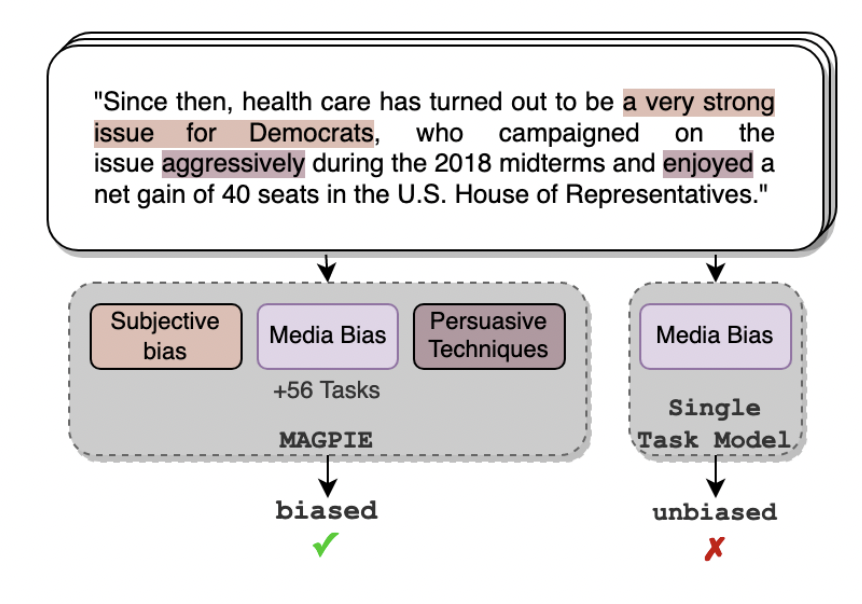
\includegraphics[width=0.9\linewidth]{images/magpie.png}
    \caption{MAGPIE containing a pre-trained representation of various biases \cite{horych-2024-magpie}.}
    \label{fig:magpie}
\end{figure}

\textbf{MAGPIE} \cite{horych-2024-magpie} is a large-scale, RoBERTa-based, multitask pre-training approach specifically designed for media bias detection, pre-fine-tuned on fifty-nine bias-related tasks covering a broad spectrum of biases. Pre-fine-tuning is a large-scale training phase situated between language model pre-training and fine-tuning. It involves extensive multitask learning (MTL) and aims to foster the development of representations that generalise more effectively across various tasks \cite{aghajanyan-2021-muppet}. Pre-fine-tuning allows multitask-approach such as MAGPIE to generalise better on various tasks related to media bias, enabling better performance on these tasks compared to single-task RoBERTa approach \cite{horych-2024-magpie}.

Unfortunately, MAGPIE is only trained to output binary classification (biased or unbiased) and mostly trained on sentences, therefore unable to be fine-tuned for article-level media bias classification task. However, the model and its feature representations can still be utilised for a feature-based approach \cite{sun-2020-fine-tune}.


\section{Chunking and Hierarchical Techniques}

\begin{figure}[htbp]
    \centering
    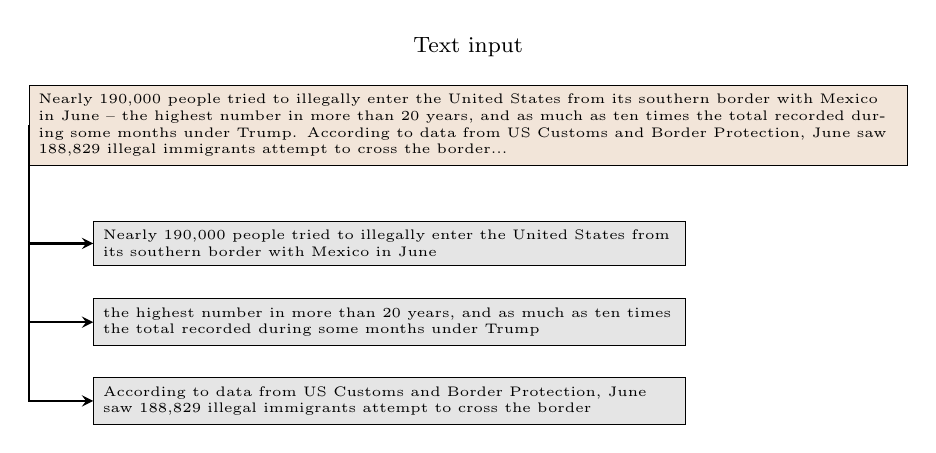
\begin{tikzpicture}
        \tikzstyle{arrow} = [thick,->,>=stealth]
        \tikzstyle{chunk} = [rectangle, draw, fill=gray!20, font=\tiny, text width=0.6\linewidth, align=left]
        \tikzstyle{label} = [text centered,font=\footnotesize]

        \node[label] at (0, 1) {Text input};
        \node (input) [draw, align=left, text width=0.9\linewidth, font=\tiny, fill=brown!20] at (0, 0) {Nearly 190,000 people tried to illegally enter the United States from its southern border with Mexico in June – the highest number in more than 20 years, and as much as ten times the total recorded during some months under Trump. According to data from US Customs and Border Protection, June saw 188,829 illegal immigrants attempt to cross the border...};

        \node[chunk] (chunk1) [draw] at (-1, -1.5) {Nearly 190,000 people tried to illegally enter the United States from its southern border with Mexico in June};
        \node[chunk] (chunk2) [draw] at (-1, -2.5) {the highest number in more than 20 years, and as much as ten times the total recorded during some months under Trump};
        \node[chunk] (chunk3) [draw] at (-1, -3.5) {According to data from US Customs and Border Protection, June saw 188,829 illegal immigrants attempt to cross the border};

        \draw[arrow] (input.west) |- (chunk1.west);
        \draw[arrow] (input.west) |- (chunk2.west);
        \draw[arrow] (input.west) |- (chunk3.west);
    \end{tikzpicture}
    \caption{Illustration of chunking}
    \label{fig:chunking}
\end{figure}


\textbf{Chunking} is a technique used to break down text into smaller, more manageable units. This technique can be applied to segment documents into smaller paragraphs or sentences, as illustrated in Figure \ref{fig:chunking}, facilitating more efficient processing and analysis. \textbf{Hierarchical models} incorporate multiple levels of abstraction or granularity to capture complex relationships within data. These models are particularly useful when dealing with structured data that naturally falls into a hierarchical organisation, such as documents composed of paragraphs and sentences. Furthermore, \textbf{hierarchical transformer model} is a variant of the transformer architecture that incorporate hierarchical structures to handle long sequences more efficiently. These models process data at different levels, such as sentences within paragraphs, to capture hierarchical relationships. Figure \ref{fig:hi_transformer} shows an example of hierarchical transformer modelused to produce document embeddings by utilising sentence-level and word-level information \cite{wu-2021-hi-transformer}.

\begin{figure}[htbp]
    \centering
    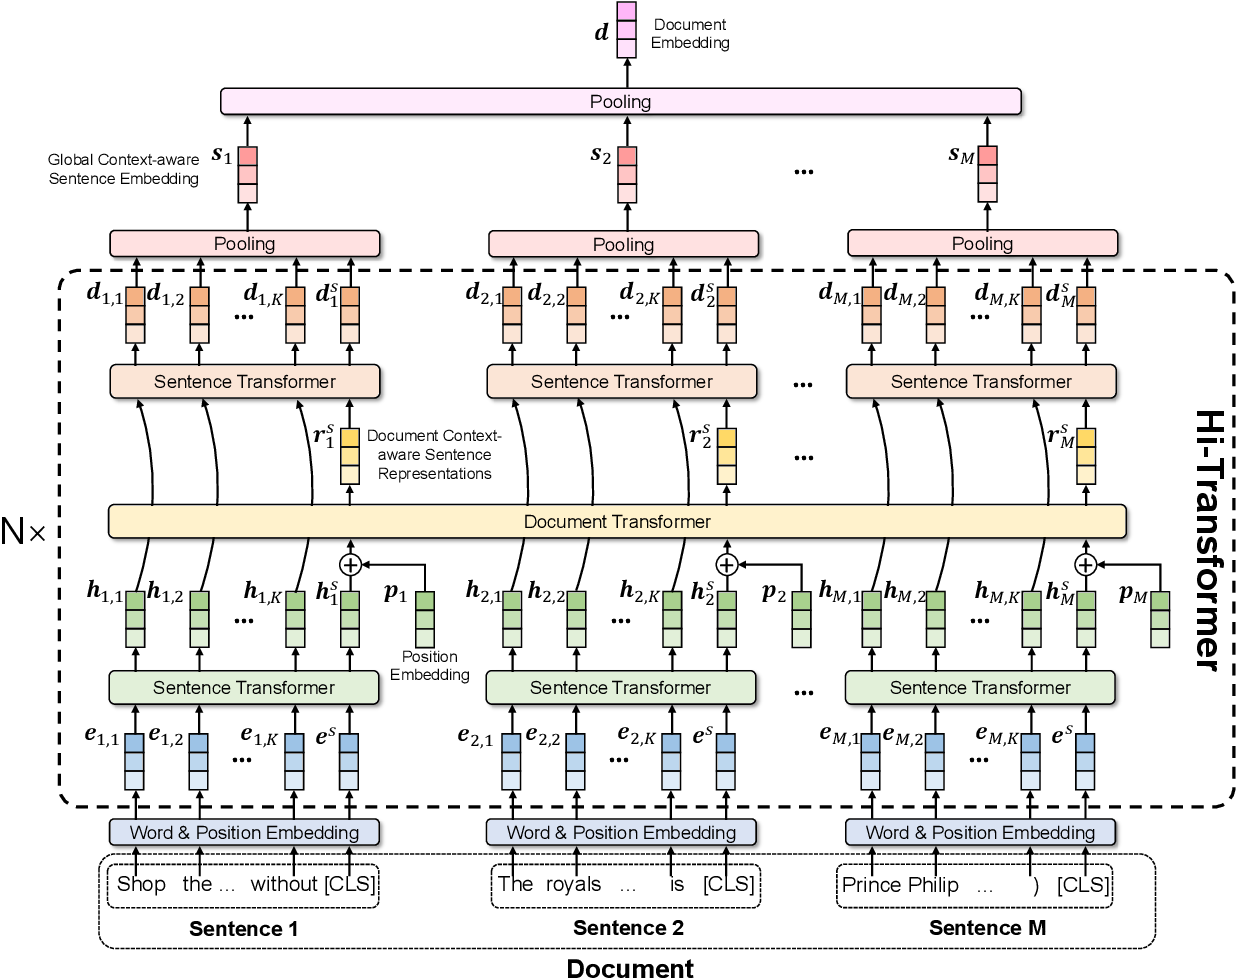
\includegraphics[width=0.9\linewidth]{images/hi_transformer.png}
    \caption{An example of hierarchical transformer model, Hi-Transformer\cite{wu-2021-hi-transformer}, to model long document}
    \label{fig:hi_transformer}
\end{figure}

\section{Document Classification}

Automatic document classification is first mentioned in 1963 \cite{borko-1963-auto-doc-classification}, with earlier text processing concepts and techniques defined in the 1950s \cite{luhn-1958-business-intelligence-system}. Document classification refers to the task of classifying text documents, commonly include large text processing and handling with various structure and content type. Typical use cases may include work with legal and financial documents, reports, and managing digital libraries.

In 2022, according to International Data Corporation (IDC) report, unstructured data accounted for 90\& of the total of organisation-generated data, in forms of purchase orders, product inventories, import/export records, sales agreements, contracts, patents, patient treatment notes, financial earning reports, and employee performance records, among many others \cite{box-2023-untapped}. Unstructured data refers to unorganised data that cannot be stored well into database, commonly in form of large collections of texts, terabytes or petabytes in size and growing exponentially \cite{mishra-2017-structured-unstructured}. Thus, the need to automatically manage and organise large amount of text and retrieve useful knowledge (knowledge discovery) is highly apparent \cite{mali-2021-relevance-of-preprocessing}.

Automatic document classification is an active area of research, with a primary focus on methods capable of handling long sequences and extracting relevant knowledge or information. Convolutional Neural Networks (CNN) \cite{afzal-deepdocclassifier,liu-2017-xmlcnn} and Hierarchical Attention Networks (HAN) \cite{yang-2016-han} have been traditionally used for this task. However, these approaches were later outperformed by DocBERT \cite{adhikari-2019-docbert}, which achieved superior results by leveraging knowledge distillation from the BERT-large model.

Straightforward, fine-tuning an encoder-based language model such as BERT is not necessarily effective for document-level processing as they are only able to process a maximum of 512 tokens, prompting significant information loss. Moreover, classification models that demonstrated significant results have been shown to perform poorly or even fail when they are tested on large documents \cite{wan-2019-long-length}.

There exist other LLMs that are designed specifically to handle longer sequences: Longformer \cite{beltagy-2020-longformer}, BigBird \cite{zaheer-2021-bigbird}. Both are hierarchical transformer models that utilises combination of global and local attention mechanisms. However, Longformer has been reported to not consistently surpass the baseline models in classification of long documents, performing only notably better than the baseline models on only two datasets \cite{park-2022-efficient}.

Several techniques have been implemented to combat the problem of handling long sequences, namely chunking and hierarchical techniques, as described previously. Pappagari et al. \cite{pappagari-2019-hierarchical} are among the first to utilise the transformer architecture for long sequences classification, introducing chunking and propagation methods. Su et al. \cite{su-2021-classifying} used chunking methods in a hierarchical transformer model with 'CLS-Pooling' (as also described in \cite{adhikari-2019-docbert}) to extract representations on the document-level for the task of clinical document classification. Khandve et al. \cite{khandve-2022-hierarchical-longdoc} also implemented a hierarchical model by utilising BERT and Bi-LSTM layers for long document classification tasks.


\section{Article-Level Media Bias Classification}

Article-level classification can be seen as a subset of document classification that specifically targets articles. This field focuses on categorising article-like texts such as news pieces, blogs, and other similar formats that typically comprise multiple paragraphs. Article-level media bias classification refers to the task of detecting and classifying media bias contained within a text. Article contents length generally falls between medium to long sequences, as they are not as lengthy as legal documents or clinical studies that typically contain multiple pages of text. Most news articles stay between several hundred to several thousand words.


\begin{comment}

\begin{figure}[htbp]
    \centering
    \fbox{
        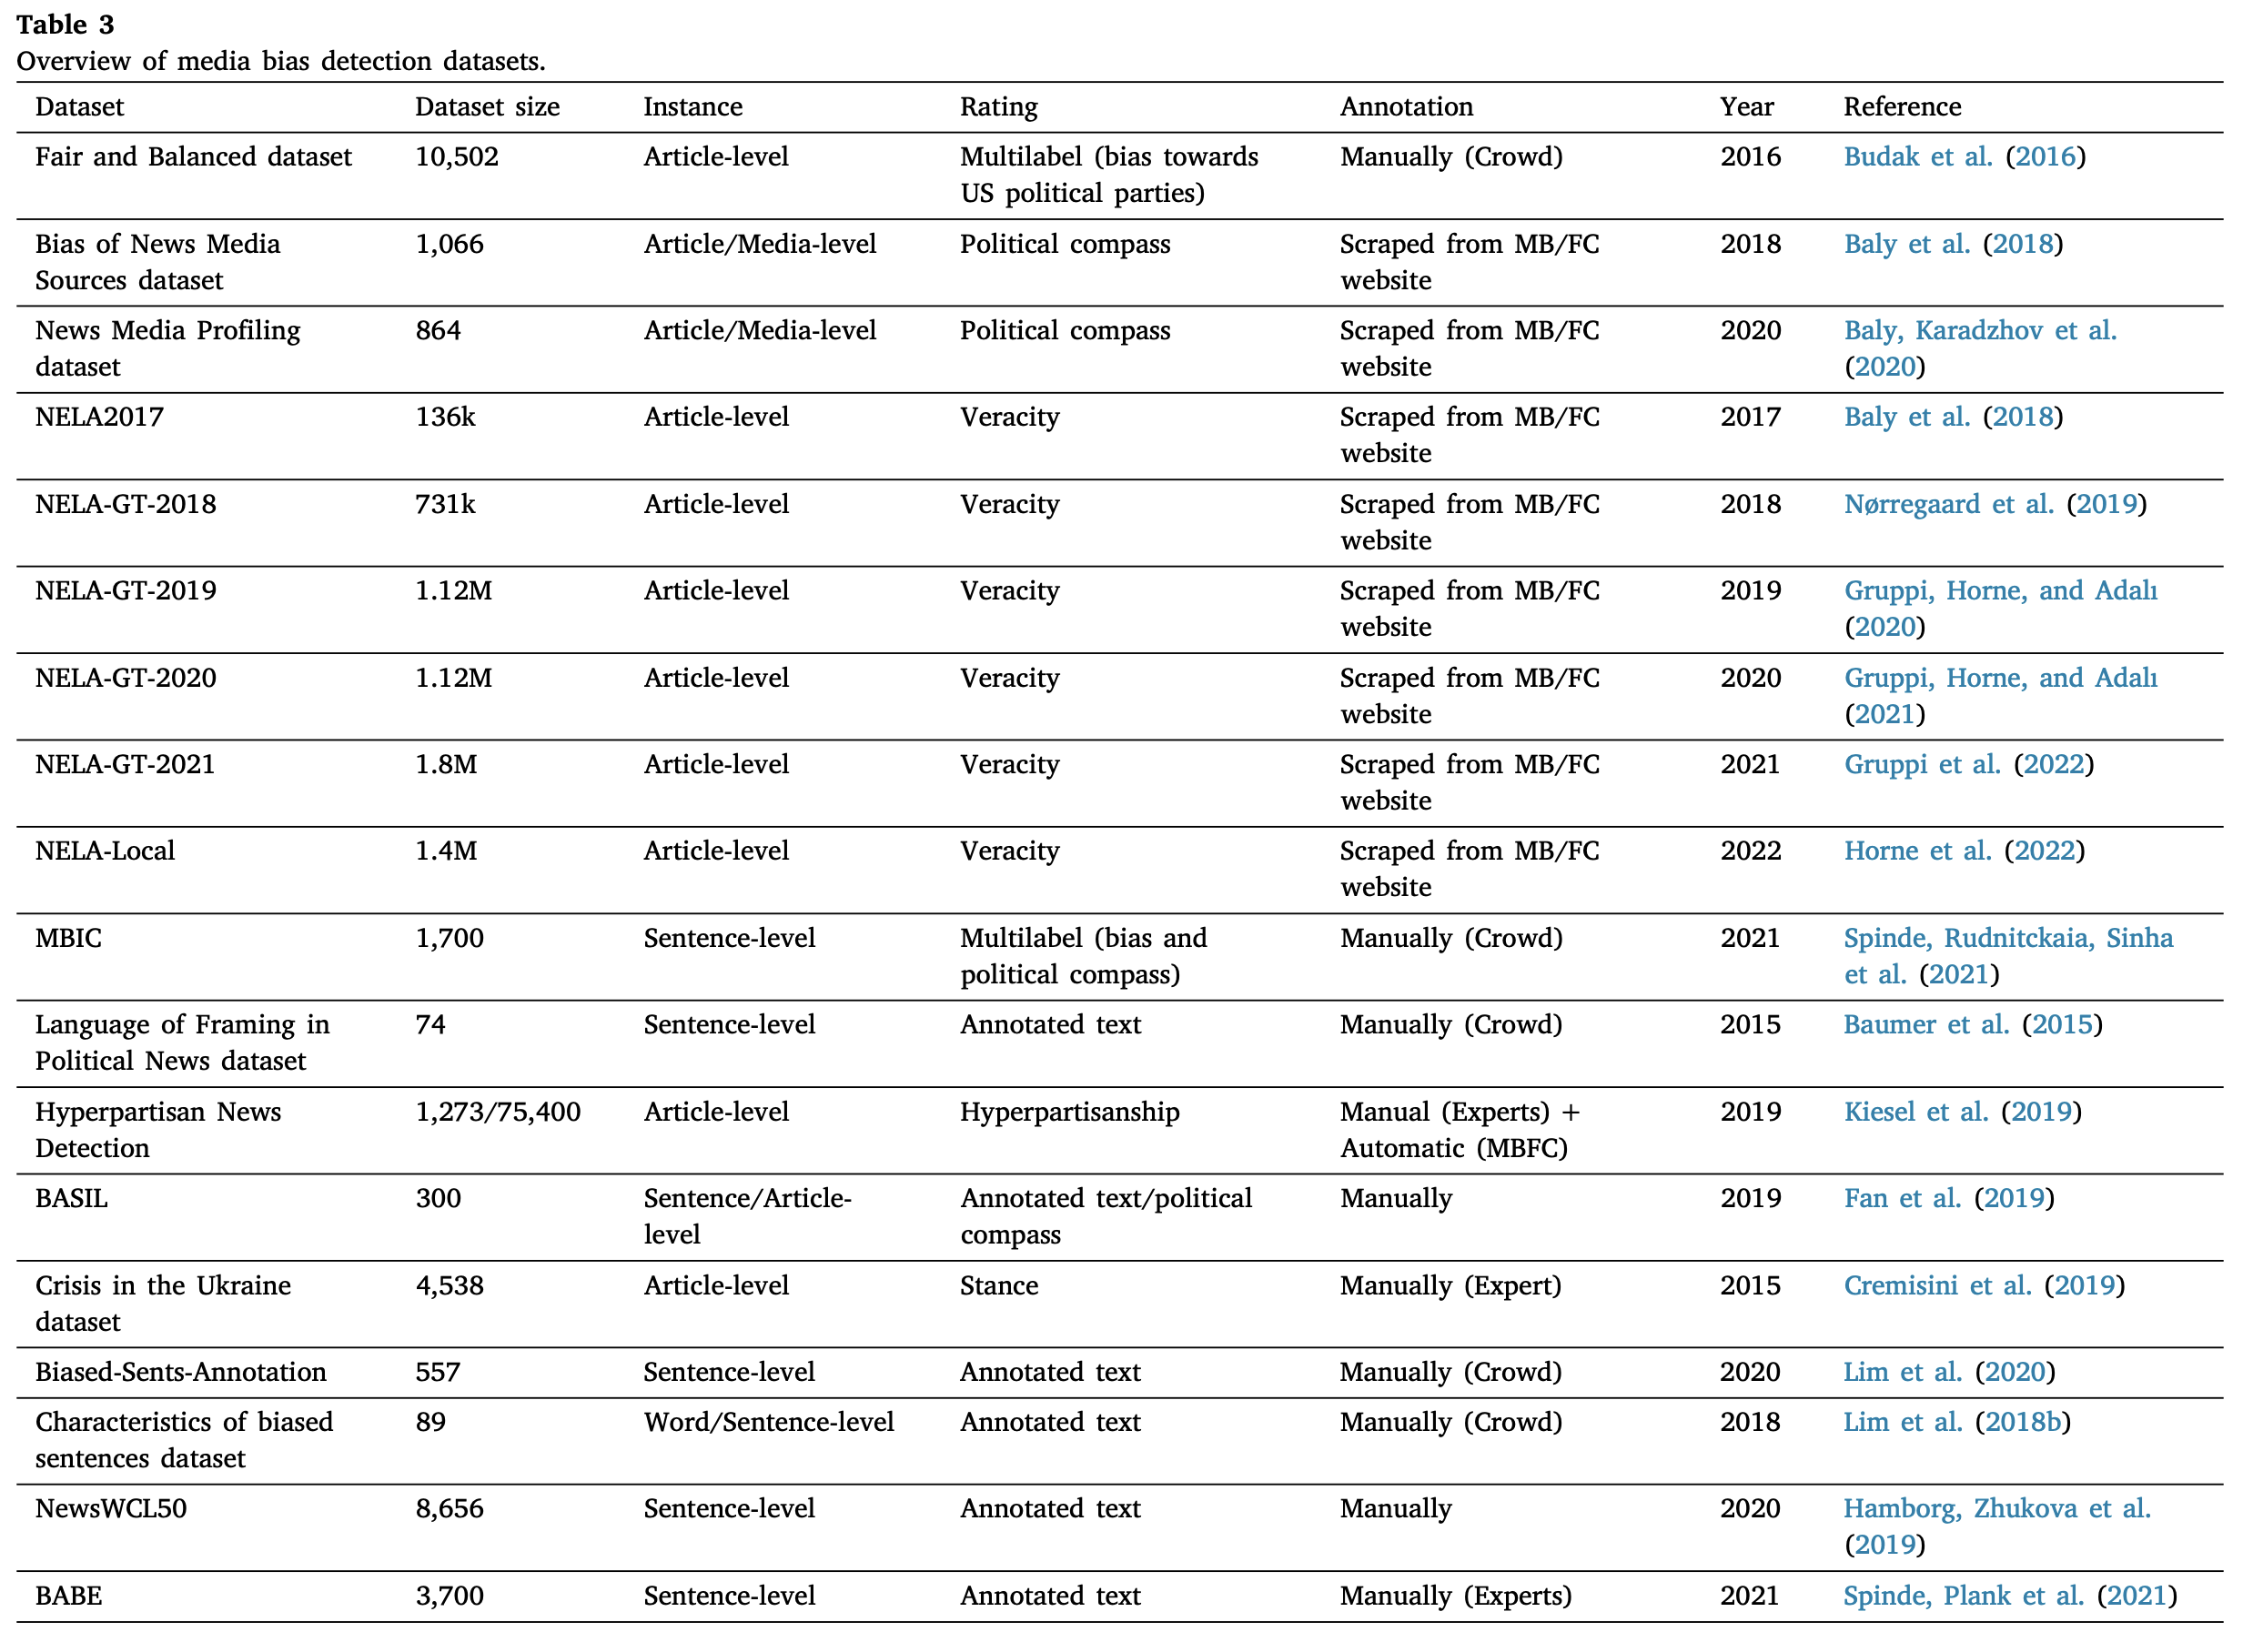
\includegraphics[width=0.9\linewidth]{images/media_bias_dataset_overview.png}}
    \caption{Overview of available media bias datasets \cite{rodrigo-2024-systematic-review-media-bias}}
    \label{fig:media-bias-dataset-overview}
\end{figure}

\end{comment}

Current available datasets for article-level and media bias classification in general are quite limited, often varying in formats or covering different types of bias. The \textbf{BASIL} dataset \cite{fan-2019-basil} is the most commonly used bias dataset, containing 300 articles with both article-level and phrase-level annotations. This dataset focuses on informational bias in news articles as it appears more frequently than lexical bias. However, the obvious drawback of this dataset is the low amount of articles included as it is not nearly enough data to get a good working detection model. \textbf{NLPCSS} \cite{chen-2020-nlpcss} (6964 articles), annotated via Ad Fontes labels, contains article-level textual content with three bias labels (bias, neutral, or unknown). Focusing on political bias and unfairness, this dataset can potentially serve as a suitable resource for an article-level media bias classification task. The \textbf{BAT} \cite{spinde-2023-bat} dataset (6345 articles, 321 outlets, Ad Fontes labels) is the most suitable for article-level bias detection as it supplies both bias-score and reliability-score for the whole article. However, the dataset itself does not supply the textual content of the articles and therefore needs to be extended, something that I have been working on as well during my Master's Thesis this and last year.

Furthermore, annotating media bias is not a straightforward task. Traditionally, this is done by hiring experts and journalists to manually read and determine how biased the content is. Here it is important to use multiple annotators to minimise introducing another form of bias towards the dataset. This comes with its own set of challenges as annotators might not always agree on biased text \cite{lim-2018-understanding}. As with \cite{spinde-2021-babe}, annotations are generally compiled and majority voted to achieve the final annotation given a particular text. Moreover, annotators' personal background moderately influenced their decisions and should be taken into consideration when building datasets, along with other factors such as topics, reading news habits, and honest mistakes \cite{spinde-2021-bias-words}. Clearly, this is not a cheap procedure and can act as a bottleneck when building a reliable media bias dataset.

Alternatively, organisations such as Allsides \cite{allsides} and Ad Fontes \cite{adfontes} have their own experts and annotations which can be crawled and exploited. Several papers and datasets \cite{spinde-2023-bat,chen-2020-nlpcss,kulkarni-2018-multi-view} have utilised this approach. However, since these datasets depend on manual labeling from third-party organisations, the selection of articles likely also introduces bias into the dataset \cite{spinde-2023-bat}.

Current State-of-the-Art (SOTA) approaches in media bias classification typically employs a transformer-based approach, either by fine-tuning or exploiting Large Language Models such as BERT \cite{devlin-2019-bert} or RoBERTa \cite{liu-2019-roberta}.

Past works on media bias classification typically use the BASIL dataset, operating on a sentence-level and outputting binary result (either biased or not) \cite{maab-2023-lexical-bias-detection, maab-2023-target-aware, guo-2022-modeling, van-den-berg-2020-context,lee-2021-unifying,lei-2022-sentence,lei-2024-event-relation}, complemented by the lack of appropriate and adequate datasets with article-level annotations \cite{demidov-2023-political-bias-classification}. Hence, \textbf{There are only a few existing studies on article-level media bias classification}. Chen et al. \cite{chen-2020-detecting-media-bias-gaussian} utilised a Gaussian mixture model, incorporating probability distributions of frequency, positions, and sequential order of lexical and informational sentence-level bias to detect article-level bias. Kulkarni et al. \cite{kulkarni-2018-multi-view} proposed a more complex model that leverages signals from multiple views to predict the political ideology of news articles, demonstrating that incorporating cues from the title, link structure, and content surpasses the state-of-the-art performance significantly. Given that automated text classification of news articles has been shown to benefit from using article segments instead of sentences as units of analysis, with preferences on supervised machine learning techniques \cite{barbera-2021-article-classification}, it may be advantageous to consider segment-length window size when developing methodologies.


%%% Local Variables: 
%%% mode: latex
%%% TeX-master: "thesis"
%%% End: 